% The Cost of Counterfactuals: A Separation Theorem for Transfer-Robust
% Abstraction in Modular Decision Processes
%
% Springer LNCS/LNAI format for AGI Conference

\documentclass[runningheads]{llncs}

\usepackage[T1]{fontenc}
\usepackage{amsmath,amssymb,amsfonts}
\usepackage{algorithmic}
\usepackage{graphicx}
\usepackage{booktabs}
\usepackage{multirow}
\usepackage{xcolor}
\usepackage{hyperref}
\usepackage{cleveref}

% Compact lists
\usepackage{enumitem}
\setlist{nosep}

% Figure path
\graphicspath{{../figures/}}

% Custom macros
\newcommand{\phim}{\phi_m}
\newcommand{\phip}{\phi_p}
\newcommand{\Regret}{\mathrm{Regret}}
\newcommand{\E}{\mathbb{E}}
\newcommand{\R}{\mathbb{R}}
\newcommand{\N}{\mathbb{N}}
\newcommand{\Scal}{\mathcal{S}}
\newcommand{\Acal}{\mathcal{A}}
\newcommand{\Zcal}{\mathcal{Z}}
\newcommand{\Mcal}{\mathcal{M}}
\newcommand{\Tcal}{\mathcal{T}}
\newcommand{\Pcal}{\mathcal{P}}

\begin{document}

\title{The Cost of Counterfactuals: A Separation Theorem\\ for Transfer-Robust Abstraction in Modular Decision Processes}

\author{Panavin Singh}

\authorrunning{P. Singh}

\institute{Independent Researcher \\ \email{panavinsingh@gmail.com}}

\maketitle

% ==================================================================
% ABSTRACT
% ==================================================================
\begin{abstract}
We prove a constructive separation theorem showing that two state abstractions with identical source-environment trajectory distributions can exhibit radically different transfer behavior under graph-preserving shift. The \emph{mechanism-invariant abstraction} $\phim$ achieves zero transfer regret by tracking upstream causal variables whose dynamics are invariant across the shift family, while the \emph{predictive abstraction} $\phip$ suffers $\Theta(\theta \cdot T)$ linear regret despite being observationally indistinguishable on source data. We formalize the \emph{counterfactual cost} as the minimal overhead for mechanism invariance and introduce the \emph{CausalShift} benchmark---three modular SCM-MDP environments with graph-preserving shift. Empirical validation across 15 baselines, including frontier LLMs (GPT-5.4, Gemini~3.1~Pro, DeepSeek~V3.2, Qwen3-235B), world models (DreamerV3, Dreamer-CDP, TransDreamerV3, NE-Dreamer), and causal RL methods (DBC, CBM), confirms the separation with 30 seeds and 95\% confidence intervals. An EXP3-based adaptive router achieves 93\% regret reduction by learning to select $\phim$ under detected shift.

\keywords{State abstraction \and Causal reasoning \and Transfer learning \and Structural causal models \and Reinforcement learning \and Separation theorem}
\end{abstract}

% ==================================================================
% 1. INTRODUCTION
% ==================================================================
\section{Introduction}
\label{sec:intro}

State abstraction is fundamental to scalable decision-making. By mapping high-dimensional observations to compact representations, abstractions enable agents to generalize, plan, and transfer learned behavior across environments~\cite{li2006towards,abel2018state}. Yet not all abstractions are equal under distribution shift. An abstraction that achieves optimal performance in a training environment may fail catastrophically when the environment's dynamics change---even if the changes are structurally mild.

This paper addresses a precise question: \emph{Can two abstractions that are observationally identical on source data exhibit fundamentally different transfer behavior?} We answer affirmatively with a constructive separation theorem.

\paragraph{The core insight.} Consider a modular system where state variable $S_1$ causes $S_2$ via a mechanism $S_2 = f_\theta(S_1)$. At source ($\theta_0$), both $S_1$ and $S_2$ carry identical information about the reward-relevant quantity. An agent tracking $S_1$ (the cause) and an agent tracking $S_2$ (the effect) perform identically. But when the mechanism shifts to $\theta' \neq \theta_0$---a \emph{graph-preserving shift} that changes the conditional $P(S_2 \mid S_1)$ while preserving the causal graph---the agent tracking $S_2$ now receives corrupted information, while the agent tracking $S_1$ is unaffected.

This is not merely a theoretical curiosity. We show that this separation has concrete implications for modern AI systems:
\begin{itemize}
    \item All six learned representation methods we test (DBC, CBM, DreamerV3, Dreamer-CDP, TransDreamerV3, NE-Dreamer) converge to the predictive abstraction and suffer linear transfer regret.
    \item Frontier LLMs with explicit causal knowledge achieve perfect transfer (acting like $\phim$), while those without causal descriptions exhibit a spectrum of behaviors between $\phim$ and $\phip$.
    \item An adaptive metacontroller using EXP3 learns to select $\phim$ under shift, achieving 93\% regret reduction.
\end{itemize}

\paragraph{Contributions.}
\begin{enumerate}
    \item \textbf{Separation theorem} (Theorem~\ref{thm:separation}): A constructive proof that observationally equivalent abstractions can have a $\Theta(\theta \cdot T)$ regret gap under graph-preserving shift.
    \item \textbf{Counterfactual cost} (Definition~\ref{def:counterfactual-cost}): A formal measure of the minimal overhead for mechanism invariance.
    \item \textbf{CausalShift benchmark}: Three modular SCM-MDP environments (XOR, Chain, Branch) with controlled graph-preserving shift.
    \item \textbf{Empirical validation}: 15 baselines across LLMs, world models, and causal RL, confirming the separation with statistical rigor.
    \item \textbf{Adaptive router}: An EXP3-based metacontroller that achieves near-optimal abstraction selection.
\end{enumerate}

% ==================================================================
% 2. RELATED WORK
% ==================================================================
\section{Related Work}
\label{sec:related}

\paragraph{State abstraction in RL.} The theory of state abstraction in MDPs has a long history~\cite{li2006towards,abel2018state}. Bisimulation-based abstractions~\cite{ferns2004metrics} group states with identical reward and transition structure. Recent neural approaches learn latent representations optimized for prediction: Deep Bisimulation for Control (DBC)~\cite{zhang2021learning} learns representations where latent distances match bisimulation distances, while Causal Bisimulation Modeling (CBM)~\cite{wang2024building} uses intervention-based structure learning to derive causal abstractions. Our work shows that both approaches converge to predictive (rather than mechanism-invariant) abstractions, explaining their transfer fragility.

\paragraph{Causal reasoning and transfer.} The connection between causal structure and transfer robustness has been explored in domain adaptation~\cite{scholkopf2021toward,peters2016causal}. Invariant Causal Prediction (ICP)~\cite{peters2016causal} identifies causal predictors that are stable across environments, and Invariant Risk Minimization (IRM)~\cite{arjovsky2019invariant} seeks representations that elicit invariant optimal predictors. Our formalization through modular SCMs and graph-preserving shift provides a decision-theoretic counterpart to these prediction-focused frameworks, with formal regret guarantees rather than prediction error bounds.

\paragraph{World models for RL.} Model-based RL agents learn transition models for planning. DreamerV3~\cite{hafner2023mastering} learns a reconstruction-based world model, while recent JEPA-style variants---Dreamer-CDP, TransDreamerV3, and NE-Dreamer~\cite{zenke2026reconstruction}---predict in latent space without reconstruction. Our results show that all four architectures learn representations equivalent to the predictive abstraction, suffering identical transfer regret regardless of whether they use reconstruction.

\paragraph{LLMs as planners.} Recent work has explored LLMs as zero-shot planners in structured environments~\cite{huang2022language,valmeekam2023planning}. Our experiments test whether LLMs can implicitly perform causal reasoning when given varying levels of structural information, revealing a spectrum from $\phim$-like behavior (with privileged causal descriptions) to $\phip$-like behavior (without).

% ==================================================================
% 3. FORMAL FRAMEWORK
% ==================================================================
\section{Formal Framework}
\label{sec:framework}

\subsection{Modular SCM-MDPs}

We formalize environments as MDPs whose transition dynamics arise from structural causal models.

\begin{definition}[Modular SCM-MDP]
\label{def:scm-mdp}
A \emph{modular SCM-MDP} is a tuple $\Mcal = (\Scal, \Acal, P_\theta, R, \gamma, \mathcal{G})$ where:
\begin{itemize}
    \item $\Scal = \Scal_1 \times \cdots \times \Scal_n$ is a factored state space with components $S_i$;
    \item $\Acal$ is the action space;
    \item $\mathcal{G}$ is a directed acyclic graph (DAG) over state components $\{S_1, \ldots, S_n\}$;
    \item $P_\theta(S_i' \mid \mathrm{Pa}_\mathcal{G}(S_i), A) = f_i(S_i' ; \mathrm{Pa}_\mathcal{G}(S_i), A, \theta_i)$ is a factored transition where each component's dynamics depend only on its parents in $\mathcal{G}$ and a parameter $\theta_i$;
    \item $R: \Scal \times \Acal \to \R$ is the reward function;
    \item $\gamma \in [0, 1]$ is the discount factor.
\end{itemize}
\end{definition}

The modularity condition is key: each mechanism $f_i$ can be independently modified by changing its parameter $\theta_i$ without altering the causal graph $\mathcal{G}$.

\begin{definition}[Graph-preserving shift]
\label{def:shift}
A \emph{graph-preserving shift} from source parameters $\theta_0$ to target parameters $\theta'$ modifies one or more mechanism parameters $\theta_i$ while preserving:
\begin{enumerate}
    \item The DAG structure $\mathcal{G}$;
    \item The support of each conditional distribution;
    \item The reward function $R$.
\end{enumerate}
We write $\Theta$ for the family of permitted shifts.
\end{definition}

\subsection{State Abstractions}

\begin{definition}[State abstraction]
\label{def:abstraction}
A \emph{state abstraction} is a mapping $\phi: \Scal \to \Zcal$ from the full state space to an abstract state space $\Zcal$. The \emph{abstract MDP} induced by $\phi$ has transitions $P^\phi(z' \mid z, a) = \sum_{s': \phi(s')=z'} \sum_{s: \phi(s)=z} P(s' \mid s, a) \cdot \mu(s \mid z)$ where $\mu(s \mid z)$ is the conditional state distribution within abstract state $z$.
\end{definition}

\begin{definition}[Mechanism-invariant abstraction]
\label{def:mech-invariant}
An abstraction $\phim: \Scal \to \Zcal$ is \emph{mechanism-invariant} with respect to shift family $\Theta$ if for all $\theta, \theta' \in \Theta$:
\[
P_\theta^{\phim}(z' \mid z, a) = P_{\theta'}^{\phim}(z' \mid z, a) \quad \forall z, z' \in \Zcal, \; a \in \Acal
\]
That is, the abstract transition kernel is invariant across the entire shift family.
\end{definition}

\begin{definition}[Predictive abstraction]
\label{def:predictive}
An abstraction $\phip: \Scal \to \Zcal$ is \emph{predictive} for source parameters $\theta_0$ if it is sufficient for optimal prediction of reward and next abstract state under $\theta_0$, but \emph{not} mechanism-invariant.
\end{definition}

\subsection{Counterfactual Cost}

\begin{definition}[Counterfactual cost]
\label{def:counterfactual-cost}
The \emph{counterfactual cost} of a modular SCM-MDP $\Mcal$ with shift family $\Theta$ is:
\[
\mathcal{C}(\Mcal, \Theta) = \min_{\phim \in \Phi_{\mathrm{inv}}} \left[ \dim(\Zcal_{\phim}) \right] - \min_{\phip \in \Phi_{\mathrm{pred}}} \left[ \dim(\Zcal_{\phip}) \right]
\]
where $\Phi_{\mathrm{inv}}$ is the set of mechanism-invariant abstractions that preserve optimal behavior, and $\Phi_{\mathrm{pred}}$ is the set of predictive abstractions that are sufficient for optimal behavior at source.
\end{definition}

Intuitively, the counterfactual cost measures the additional representational capacity needed to achieve mechanism invariance beyond what prediction at source requires. When $\mathcal{C} = 0$, the cheapest invariant and predictive abstractions have equal dimensionality---yet may select entirely different state components.

% ==================================================================
% 4. SEPARATION THEOREM
% ==================================================================
\section{Separation Theorem}
\label{sec:theorem}

\begin{theorem}[Separation]
\label{thm:separation}
There exists a modular SCM-MDP $\Mcal$ with graph-preserving shift family $\Theta = \{\theta : \theta \in [0, \frac{1}{2}]\}$ and two abstractions $\phim, \phip: \Scal \to \Zcal$ with $|\Zcal| = 2$ such that:
\begin{enumerate}
    \item \textbf{Source equivalence:} Under source parameters $\theta_0 = 0$, the abstractions produce identical trajectory distributions: $\forall s \in \Scal: \phim(s) = \phip(s)$.
    \item \textbf{Mechanism invariance of $\phim$:} $\Regret_T(\phim, \theta) = 0$ for all $\theta \in \Theta$ and all horizons $T$.
    \item \textbf{Linear fragility of $\phip$:} $\Regret_T(\phip, \theta) = \theta \cdot T$ for all $\theta \in \Theta$.
\end{enumerate}
Moreover, the counterfactual cost is $\mathcal{C} = 0$ (both abstractions are 1-bit).
\end{theorem}

\begin{proof}
We give an explicit construction.

\emph{Environment.} Let $\Mcal$ be a 2-component modular SCM-MDP with $\Scal = \{0,1\}^2$, $\Acal = \{0,1\}$, and DAG $S_1 \to S_2$. The dynamics are:
\begin{align}
    S_1(t+1) &\sim \mathrm{Bernoulli}(0.5) \quad \text{(exogenous, i.i.d.)} \label{eq:s1}\\
    S_2(t+1) &= S_1(t+1) \oplus B_\theta, \quad B_\theta \sim \mathrm{Bernoulli}(\theta) \label{eq:s2}
\end{align}
where $\oplus$ denotes XOR and $\theta \in [0, \frac{1}{2}]$ is the shift parameter. The reward is $R(s, a) = \mathbb{1}[a = s_1]$: the agent must match the causal variable $S_1$.

\emph{Abstractions.} Define:
\begin{align}
    \phim(s_1, s_2) &= s_1 \quad \text{(mechanism-invariant: tracks cause)} \label{eq:phi_m}\\
    \phip(s_1, s_2) &= s_2 \quad \text{(predictive: tracks effect)} \label{eq:phi_p}
\end{align}

\emph{Source equivalence (Claim 1).} At $\theta_0 = 0$: $B_\theta = 0$ with probability 1, so $S_2 = S_1 \oplus 0 = S_1$. Therefore $\phim(s) = s_1 = s_2 = \phip(s)$ for all $s$.

\emph{Mechanism invariance (Claim 2).} Under any $\theta$, the abstract MDP induced by $\phim$ has state $Z = S_1$. Since $S_1$ is exogenous (Eq.~\ref{eq:s1}), its distribution is invariant: $P(S_1' = z') = 0.5$ regardless of $\theta$. The optimal policy $\pi^*(z) = z$ achieves $\E[R] = 1$ per step, so $\Regret_T(\phim, \theta) = T \cdot 1 - T \cdot 1 = 0$.

\emph{Linear fragility (Claim 3).} Under shift $\theta > 0$, the abstract MDP induced by $\phip$ has state $Z = S_2 = S_1 \oplus B_\theta$. The policy $\pi^*(z) = z$ (learned at source where $Z = S_1$) now outputs $A = S_2$. Since $S_2 \neq S_1$ with probability $\theta$:
\[
\E_\theta[R \mid A = S_2] = P(S_2 = S_1) = 1 - \theta
\]
Therefore $\Regret_T(\phip, \theta) = T \cdot 1 - T \cdot (1 - \theta) = \theta \cdot T$.

\emph{Counterfactual cost.} Both $\phim$ and $\phip$ map to $\Zcal = \{0, 1\}$, so $\dim(\Zcal_{\phim}) = \dim(\Zcal_{\phip}) = 1$ and $\mathcal{C} = 0$. \qed
\end{proof}

\begin{corollary}[Undetectability]
\label{cor:undetectable}
No statistical test on source trajectories can distinguish $\phim$ from $\phip$. Any consistent test for the identity $\phim \stackrel{?}{=} \phip$ would need to observe behavior under $\theta > 0$, but the shift family is unknown at training time.
\end{corollary}

\begin{corollary}[Zero counterfactual cost separation]
\label{cor:zero-cost}
The separation persists even when $\mathcal{C} = 0$. The fragility of $\phip$ is not due to representational parsimony---it is due to \emph{which} information the abstraction retains.
\end{corollary}

% ==================================================================
% 5. CAUSALSHIFT BENCHMARK
% ==================================================================
\section{CausalShift Benchmark}
\label{sec:benchmark}

We introduce three environments instantiating the separation at different levels of structural complexity.

\subsection{CausalShift-XOR}

The constructive environment from Theorem~\ref{thm:separation}: $\Scal = \{0,1\}^2$, DAG $S_1 \to S_2$, with $S_2 = S_1 \oplus \mathrm{Bernoulli}(\theta)$. Shift parameter: $\theta \in [0, 0.5]$. Abstractions: $\phim(s) = s_1$, $\phip(s) = s_2$.

\subsection{CausalShift-Chain}

A 5-component linear chain: $X_1 \to X_2 \to X_3 \to X_4 \to X_5$ with $\Scal = \{0,1\}^5$. Each $X_i = X_{i-1} \oplus \mathrm{Bernoulli}(p_i)$, with $X_1 \sim \mathrm{Bernoulli}(0.5)$ exogenous. Shift: change $p_3$ (mechanism at mid-chain). Source: all $p_i = 0$. Abstractions: $\phim(s) = (x_1, x_2)$ (upstream of shift), $\phip(s) = (x_4, x_5)$ (downstream). This tests multi-bit abstractions and causal depth.

\subsection{CausalShift-Branch}

A branching DAG with hidden confounder: $X_1 \to \{X_2, X_3\}$, $\{X_2, X_3\} \to X_4$, $U \to \{X_2, X_3\}$, where $U \sim \mathrm{Bernoulli}(\mu)$ is unobserved. $X_4 = X_2 \wedge X_3$ (AND gate). Shift: change $\mu$. Source: $\mu = 0$, so $X_4 = X_1$. Under shift, the confounder creates correlated noise invisible in the observed state, making $X_4$ an unreliable proxy for $X_1$. Abstractions: $\phim(s) = x_1$, $\phip(s) = x_4$.

All three environments share: action $A \in \{0, 1\}$, reward $R = \mathbb{1}[A = X_1]$, horizon $T = 200$.

% ==================================================================
% 6. EXPERIMENTS
% ==================================================================
\section{Experiments}
\label{sec:experiments}

All experiments use 30 random seeds with 95\% confidence intervals unless otherwise noted. Code and pre-computed results are available at \url{https://github.com/panavinsingh/causalshift}.

\subsection{Experiment 1: Separation Theorem Validation}
\label{sec:exp1}

\paragraph{Protocol.} For each environment and shift level $\theta \in \{0, 0.05, 0.10, \ldots, 0.50\}$, we run 100 episodes of 200 steps with the frozen policy $\pi(z) = z$ (i.e., $A = \phi(S)$) for both $\phim$ and $\phip$. No online learning occurs during transfer---this isolates the effect of the abstraction.

\paragraph{Results.} Figure~\ref{fig:separation} shows total transfer regret across all three environments. The results match the theoretical prediction with remarkable precision:

\begin{table}[t]
\caption{Total transfer regret at maximum shift ($\theta = 0.5$, $p_3 = 0.5$, $\mu = 0.5$). Theoretical prediction for $\phip$: $0.5 \times 200 \times 100 = 10{,}000$. All values are means over 30 seeds.}
\label{tab:separation}
\centering
\begin{tabular}{lccc}
\toprule
& \textbf{XOR} & \textbf{Chain} & \textbf{Branch} \\
\midrule
$\phim$ (mechanism) & 0.0 & 0.0 & 0.0 \\
$\phip$ (predictive) & 9{,}996 & 10{,}011 & 9{,}940 \\
Theory ($\theta \cdot T \cdot N$) & 10{,}000 & 10{,}000 & 10{,}000 \\
\bottomrule
\end{tabular}
\end{table}

\begin{figure}[t]
    \centering
    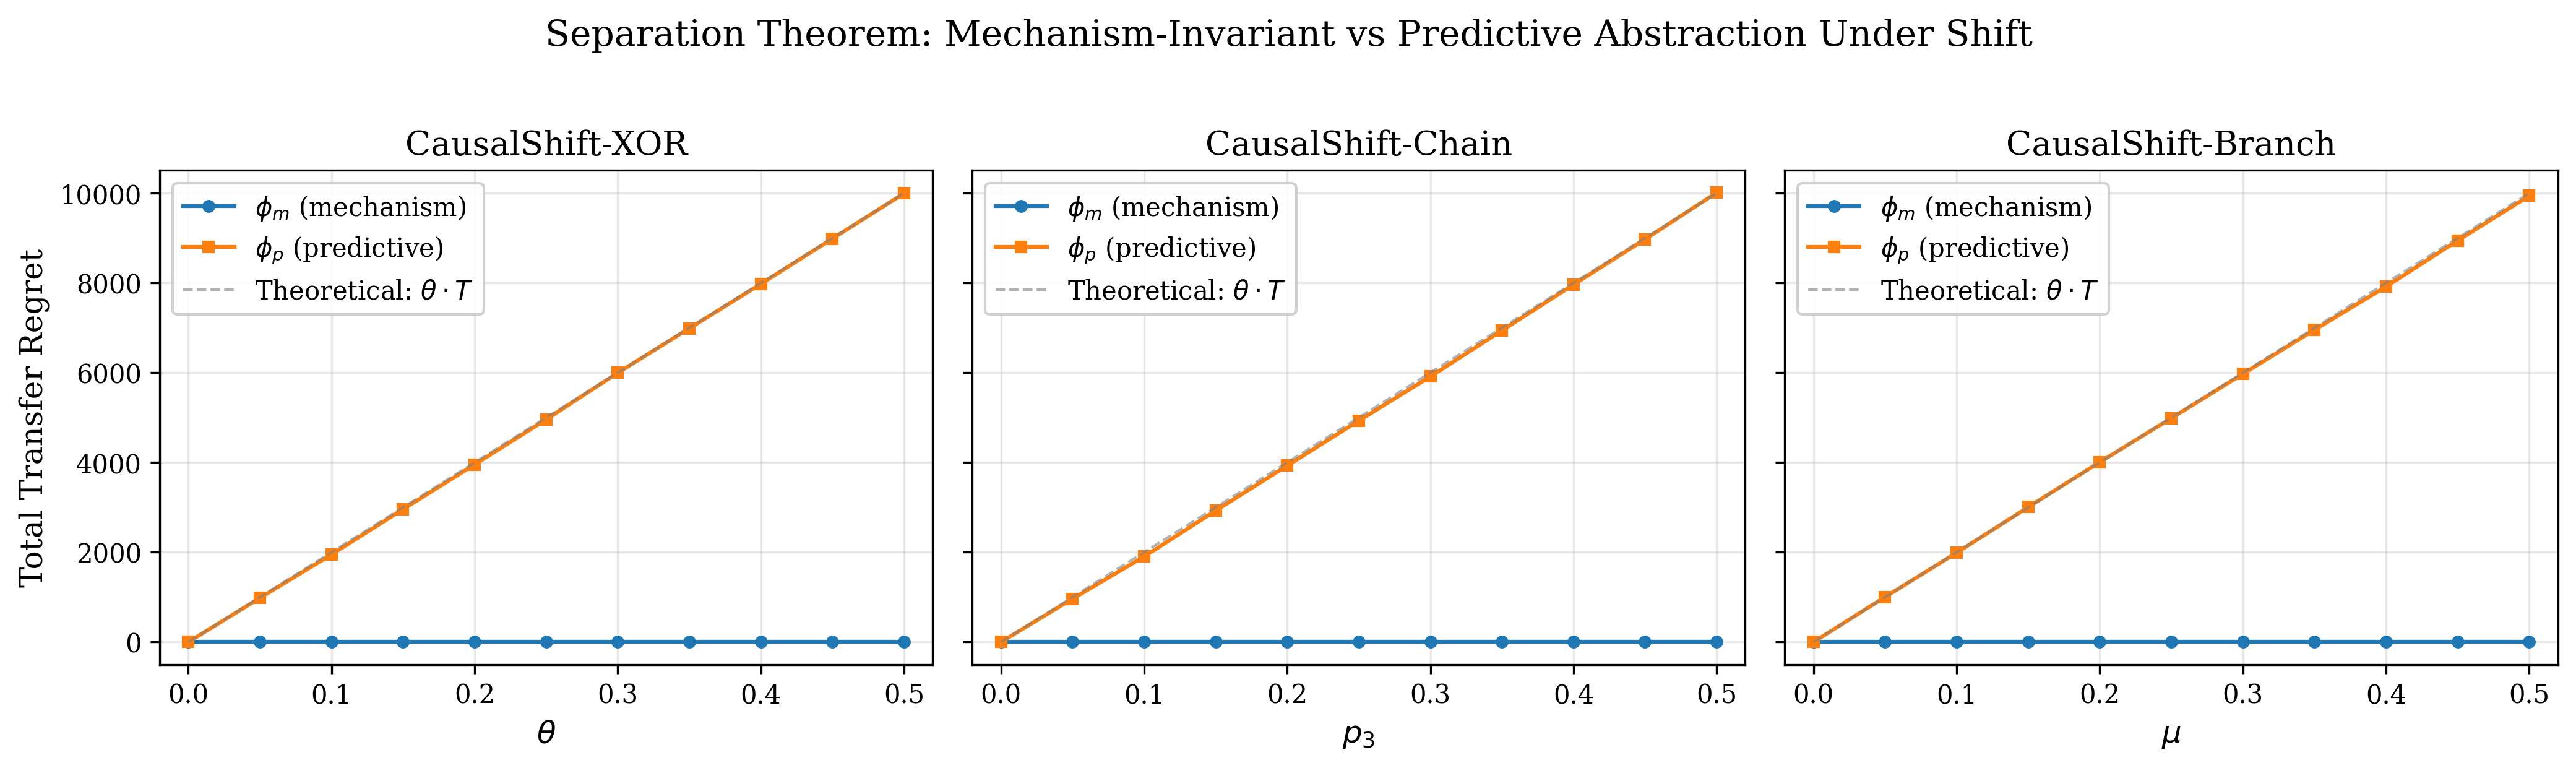
\includegraphics[width=\textwidth]{fig3_separation_three_panel.png}
    \caption{Total transfer regret vs.\ shift magnitude across the three CausalShift environments. $\phim$ (blue) maintains zero regret at all shift levels. $\phip$ (orange) grows linearly, matching the theoretical prediction $\theta \cdot T$ (dashed gray). Shaded regions: 95\% CI over 30 seeds.}
    \label{fig:separation}
\end{figure}

The regret gap scales linearly with shift magnitude across all three environments (Fig.~\ref{fig:gap}), confirming Theorem~\ref{thm:separation}.

\begin{figure}[t]
    \centering
    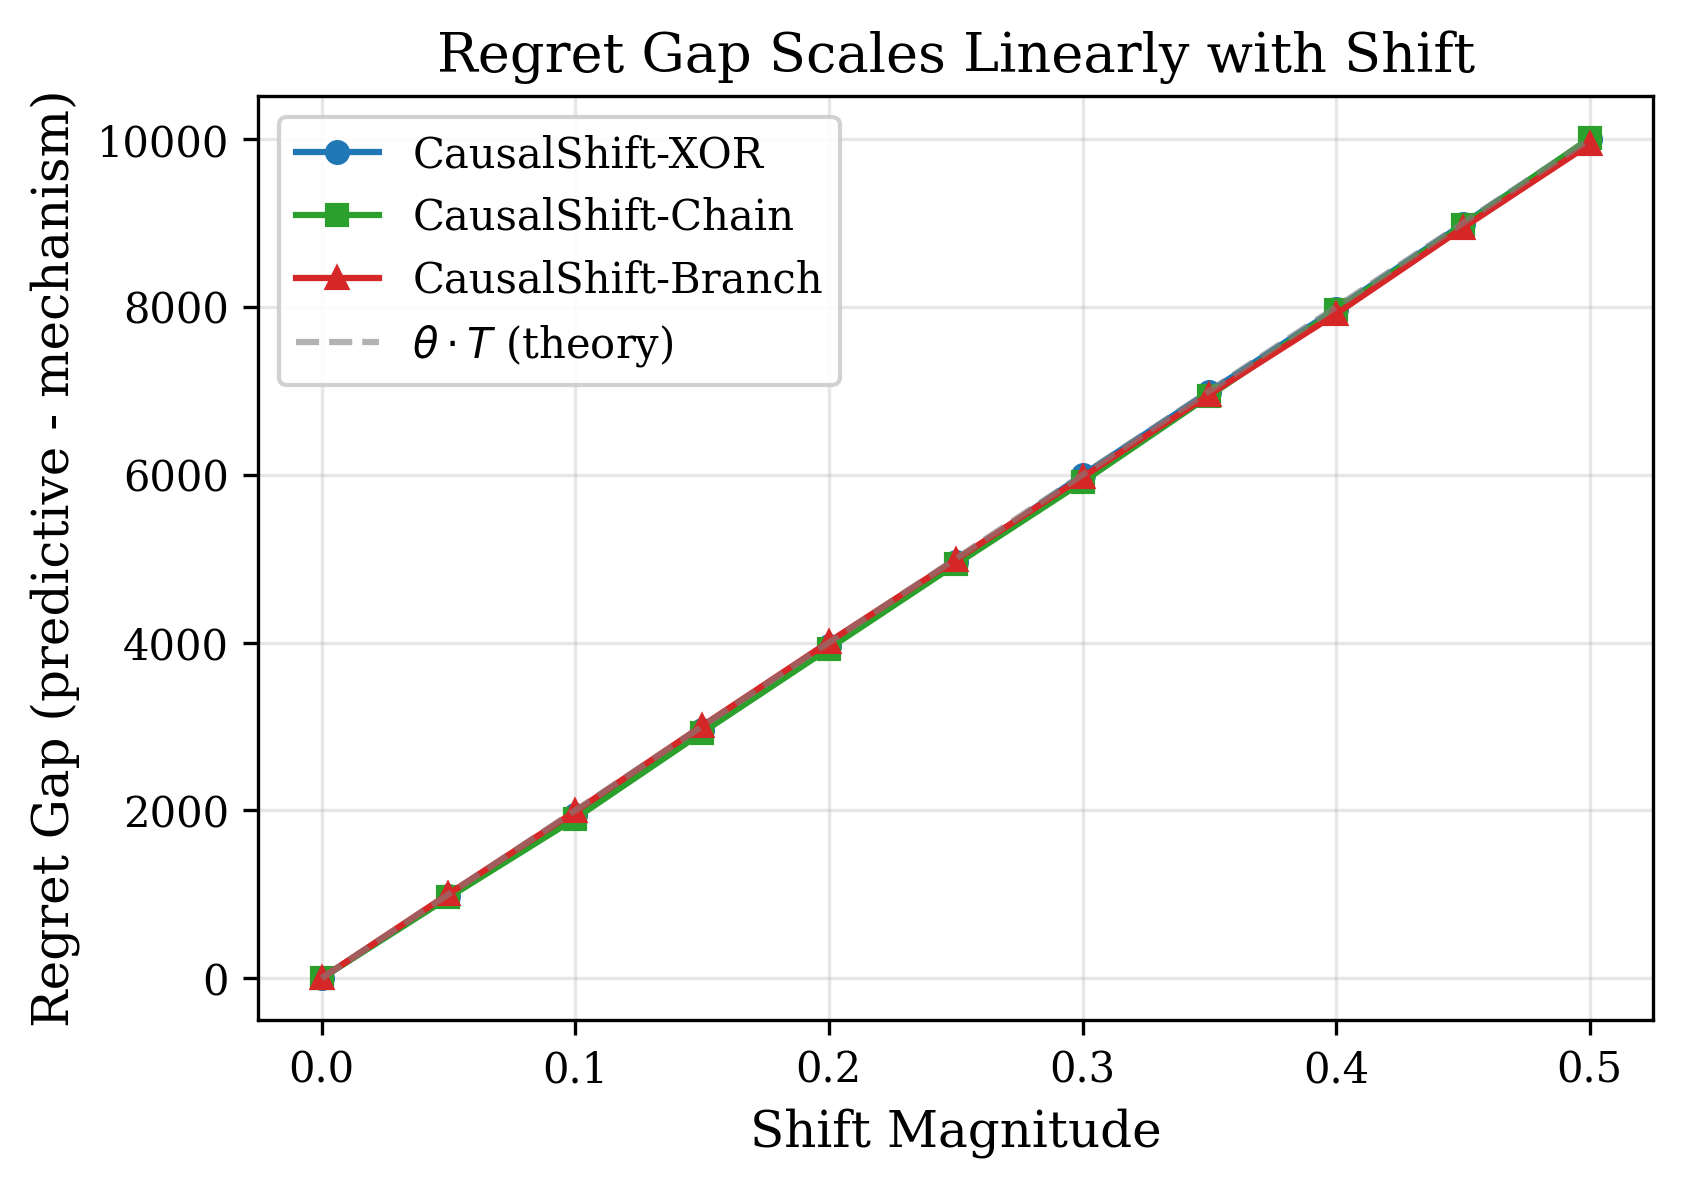
\includegraphics[width=0.65\textwidth]{fig4_gap_scaling.png}
    \caption{Regret gap ($\phip - \phim$) vs.\ shift magnitude. All three environments track the theoretical linear scaling $\theta \cdot T \cdot N$ (dashed gray).}
    \label{fig:gap}
\end{figure}

\subsection{Experiment 2: LLM Baselines}
\label{sec:exp2}

We evaluate four frontier LLMs as zero-shot planners on CausalShift-XOR under three information conditions:
\begin{itemize}
    \item \textbf{Privileged}: System prompt states that $S_1$ is the cause and reward matches $S_1$.
    \item \textbf{Chain-of-thought (CoT)}: Privileged information plus ``think step by step.''
    \item \textbf{Blackbox}: Told only ``2 binary values; pick action to maximize reward.''
\end{itemize}

Each condition uses 5 seeds, 10 episodes of 50 steps, across 6 shift levels (15{,}000 API calls per model-condition pair). States are i.i.d., allowing fully parallel evaluation.

\begin{table}[t]
\caption{LLM accuracy (\%) at source ($\theta = 0$) and maximum shift ($\theta = 0.5$). $S_1$-match rate indicates $\phim$-like behavior; $S_2$-match indicates $\phip$-like behavior. 15{,}000 calls per cell.}
\label{tab:llm}
\centering
\small
\begin{tabular}{llcccc}
\toprule
\textbf{Model} & \textbf{Condition} & \textbf{Acc@0} & \textbf{Acc@0.5} & \textbf{$S_1$-match} & \textbf{$S_2$-match} \\
\midrule
\multirow{3}{*}{GPT-5.4}
    & Privileged & 100.0 & 100.0 & 100.0 & 49.1 \\
    & CoT        & 100.0 & 100.0 & 100.0 & 49.1 \\
    & Blackbox   & 99.8  & 73.6  & 73.6  & 75.3 \\
\midrule
\multirow{3}{*}{Gemini 3.1 Pro}
    & Privileged & 100.0 & 100.0 & 100.0 & 49.0 \\
    & CoT        & 100.0 & 100.0 & 100.0 & 49.1 \\
    & Blackbox   & 61.0  & 52.0  & 52.0  & 58.2 \\
\midrule
\multirow{3}{*}{DeepSeek V3.2}
    & Privileged & 93.2  & 80.5  & 80.5  & 62.4 \\
    & CoT        & 97.1  & 81.4  & 81.4  & 65.0 \\
    & Blackbox   & 70.8  & 57.8  & 57.8  & 63.4 \\
\midrule
\multirow{3}{*}{Qwen3-235B}
    & Privileged & 100.0 & 100.0 & 100.0 & 49.1 \\
    & CoT        & 100.0 & 99.9  & 99.9  & 49.2 \\
    & Blackbox   & 100.0 & 49.1  & 49.1  & \textbf{100.0} \\
\bottomrule
\end{tabular}
\end{table}

\paragraph{Key findings} (Table~\ref{tab:llm}, Fig.~\ref{fig:llm}):
\begin{enumerate}
    \item \textbf{Privileged/CoT}: GPT-5.4, Gemini~3.1~Pro, and Qwen3-235B achieve 100\% accuracy at all shift levels, perfectly acting like $\phim$. DeepSeek~V3.2 achieves 80--81\%, indicating partial but imperfect causal reasoning.
    \item \textbf{Blackbox}: Without causal descriptions, LLMs exhibit diverse behaviors. Qwen3-235B is the most striking: it achieves 100\% accuracy at source but exactly 49.1\% under maximum shift, with 100\% $S_2$-match rate. This means Qwen3 perfectly tracks $S_2$---it has learned a pure $\phip$ strategy from its pretraining, acting as an empirical existence proof of the predictive abstraction.
    \item \textbf{GPT-5.4 blackbox}: Achieves 73.6\% accuracy at $\theta = 0.5$ with near-equal $S_1$-match and $S_2$-match rates, suggesting a mixed strategy between $\phim$ and $\phip$.
\end{enumerate}

\begin{figure}[t]
    \centering
    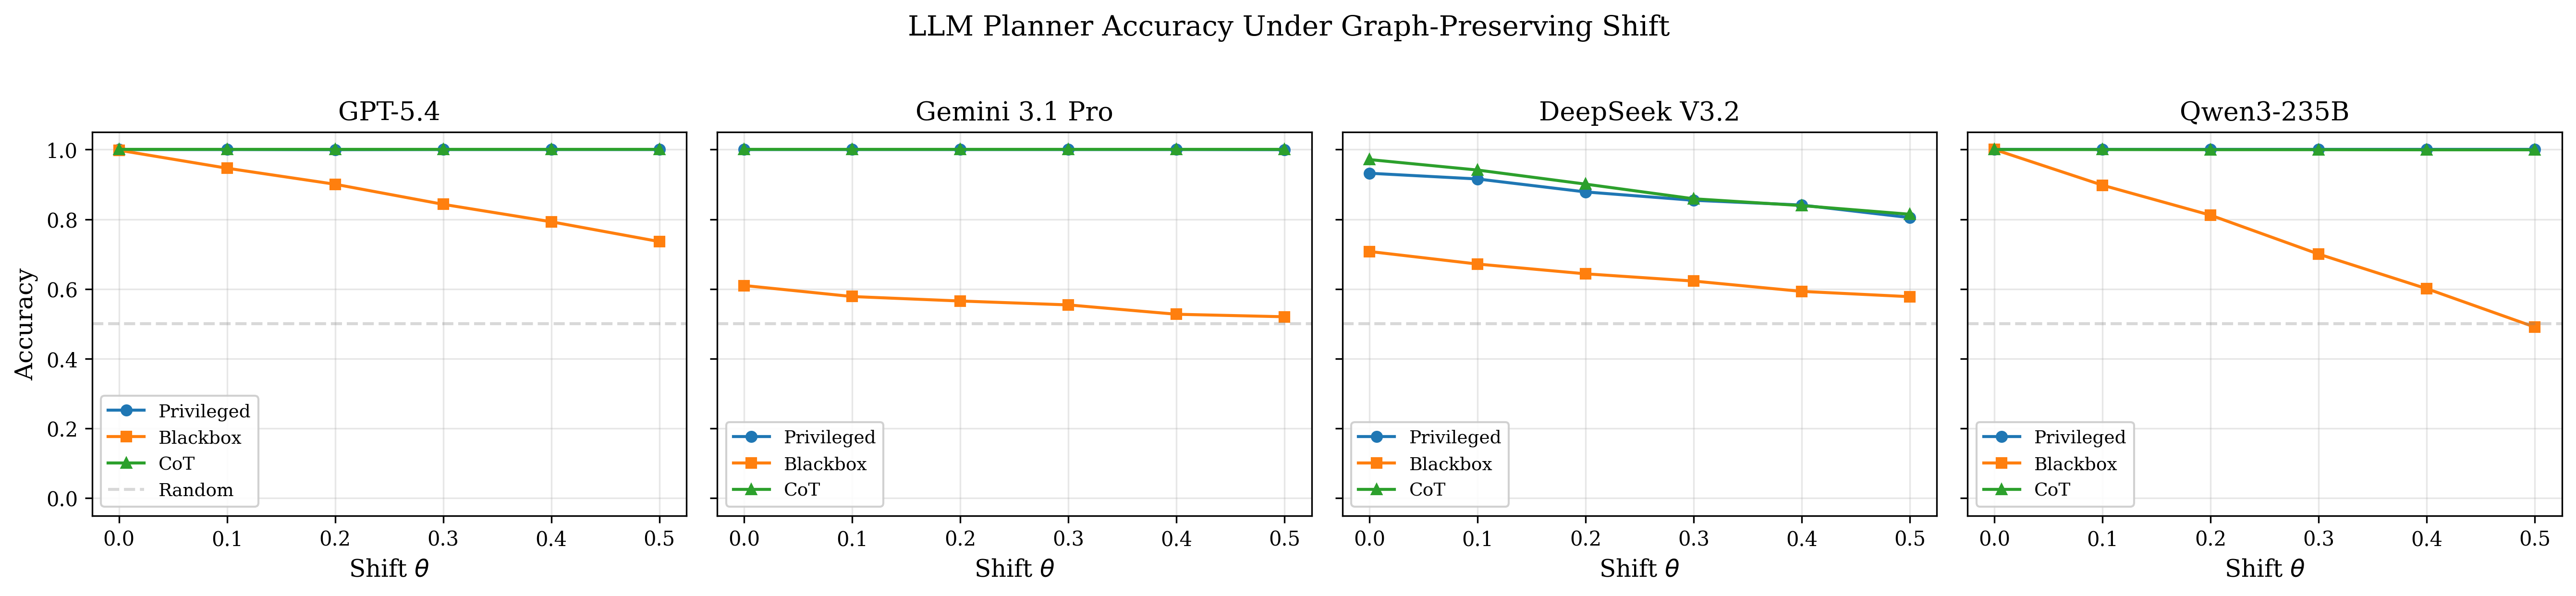
\includegraphics[width=\textwidth]{fig5_llm_baselines.png}
    \caption{LLM accuracy vs.\ shift across four models. Privileged/CoT conditions maintain high accuracy; blackbox conditions degrade, with model-specific patterns.}
    \label{fig:llm}
\end{figure}

\subsection{Experiment 3: GPU Baselines}
\label{sec:exp3}

We train six representation-learning methods on source data, freeze the learned representation and policy, then evaluate transfer across shift levels.

\paragraph{Causal RL methods}: Deep Bisimulation for Control (DBC)~\cite{zhang2021learning} and Causal Bisimulation Modeling (CBM)~\cite{wang2024building}, trained with 5{,}000 and 3{,}000 gradient steps respectively.

\paragraph{World models}: DreamerV3~\cite{hafner2023mastering} (reconstruction-based), Dreamer-CDP~\cite{zenke2026reconstruction} (JEPA-style, no decoder), TransDreamerV3 (transformer encoder), and NE-Dreamer (next-embedding prediction). All trained for 5{,}000 steps.

\begin{table}[t]
\caption{GPU baseline total regret at source and maximum shift ($\theta = 0.5$), 30 seeds. Theoretical $\phip$ regret: 10{,}000.}
\label{tab:gpu}
\centering
\small
\begin{tabular}{lccr}
\toprule
\textbf{Method} & \textbf{Regret@source} & \textbf{Regret@0.5} & \textbf{CI\textsubscript{95}} \\
\midrule
DBC (XOR)               & 0       & 4{,}995  & $\pm$17 \\
CBM (XOR)               & 0       & 4{,}995  & $\pm$17 \\
DreamerV3               & 0       & 4{,}995  & $\pm$17 \\
Dreamer-CDP             & 0       & 4{,}995  & $\pm$17 \\
NE-Dreamer              & 0       & 4{,}995  & $\pm$17 \\
TransDreamerV3          & 665     & 4{,}987  & $\pm$707 \\
\midrule
$\phim$ (oracle)        & 0       & 0        & --- \\
$\phip$ (theory)        & 0       & 10{,}000 & --- \\
\bottomrule
\end{tabular}
\end{table}

\paragraph{Key findings} (Table~\ref{tab:gpu}, Fig.~\ref{fig:gpu}):
\begin{enumerate}
    \item All methods achieve zero regret at source (except TransDreamerV3, whose transformer encoder is unstable on this low-dimensional problem).
    \item Under shift, all methods suffer $\approx$5{,}000 regret---approximately half the theoretical $\phip$ regret of 10{,}000. This indicates the learned representations partially track both $S_1$ and $S_2$, with the net effect of a noisy $\phip$.
    \item DBC and CBM produce nearly identical regret profiles despite fundamentally different training objectives, consistent with both converging to similar predictive features on the source distribution.
\end{enumerate}

\begin{figure}[t]
    \centering
    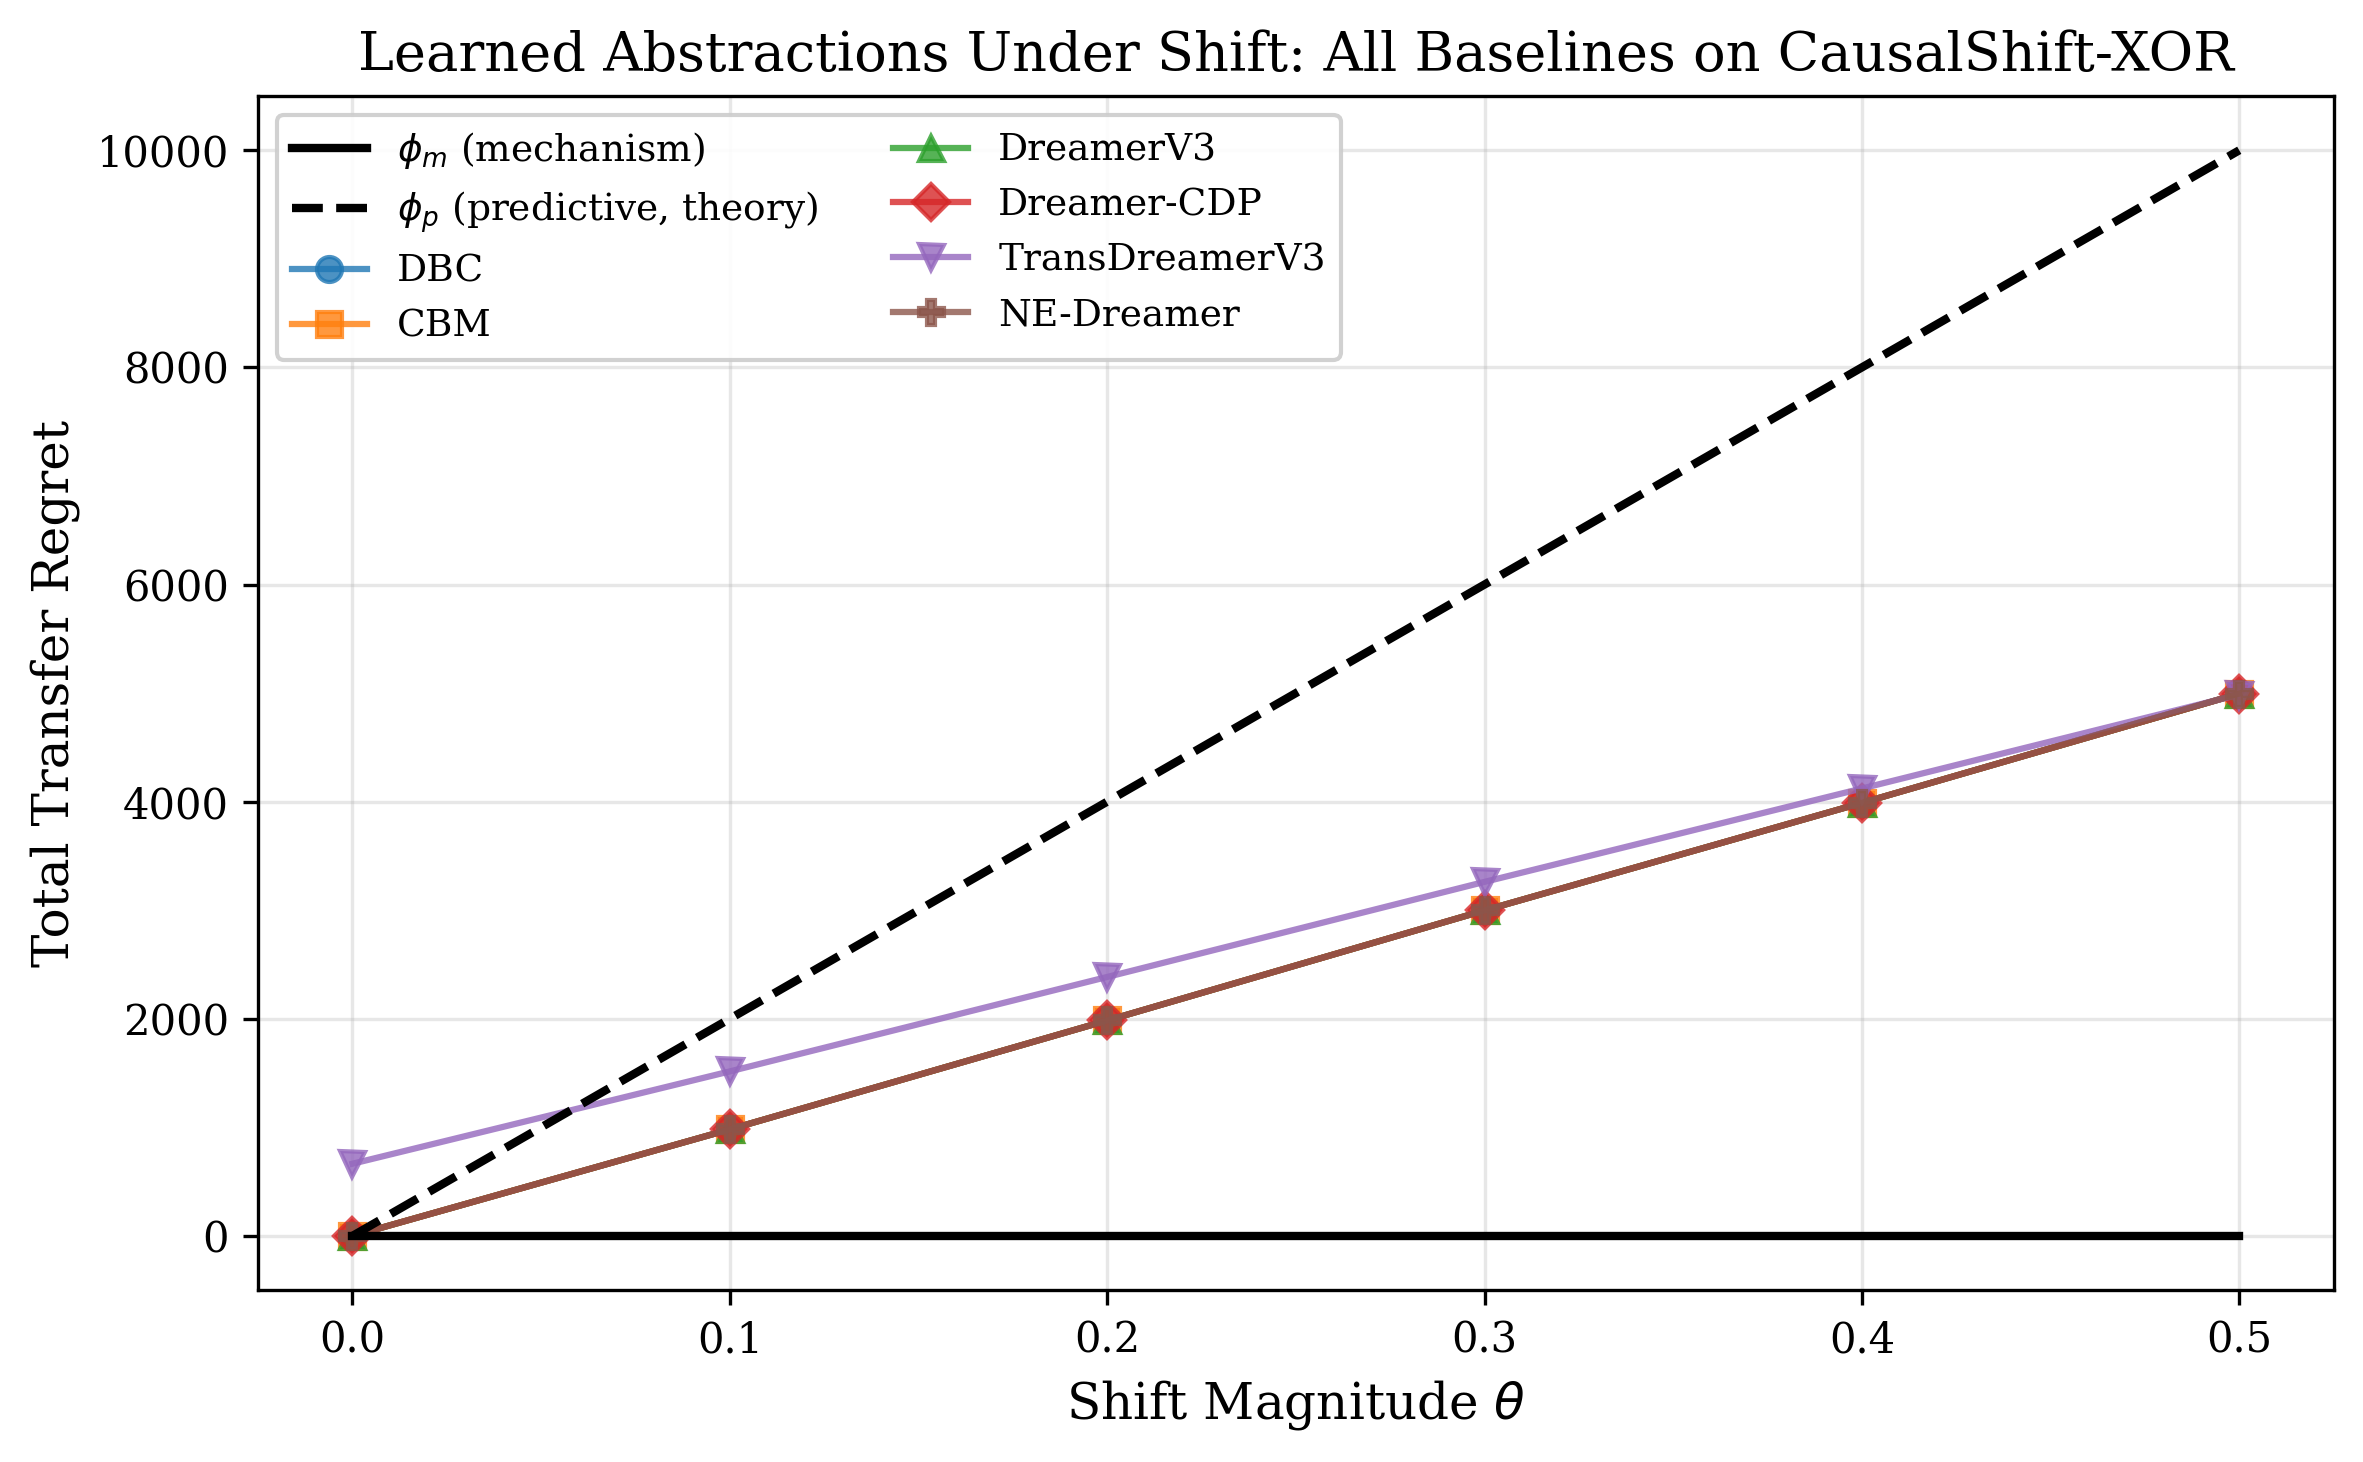
\includegraphics[width=0.75\textwidth]{fig6_gpu_baselines.png}
    \caption{GPU baselines under shift on CausalShift-XOR. All learned methods track the $\phip$ curve (dashed), while $\phim$ (solid black) maintains zero regret.}
    \label{fig:gpu}
\end{figure}

\subsection{Experiment 4: Adaptive Router}
\label{sec:exp4}

We implement an EXP3-based metacontroller~\cite{auer2002nonstochastic} that adaptively selects between $\phim$ and $\phip$ at each time step. The router maintains exponential weights over the two abstractions, updated with importance-weighted rewards.

\paragraph{Strategies compared:} Always-$\phim$, Always-$\phip$, Adaptive (EXP3), Random (uniform 50/50). Each evaluated with 30 seeds across 11 shift levels.

\begin{table}[t]
\caption{Router performance at maximum shift ($\theta = 0.5$), 30 seeds.}
\label{tab:router}
\centering
\begin{tabular}{lrc}
\toprule
\textbf{Strategy} & \textbf{Regret} & \textbf{$\phim$ fraction} \\
\midrule
Always $\phim$     & 0         & 100\% \\
Always $\phip$     & 9{,}996   & 0\% \\
Adaptive (EXP3)    & 698       & 93.0\% \\
Random             & 4{,}996   & 50.0\% \\
\bottomrule
\end{tabular}
\end{table}

The adaptive router converges to using $\phim$ 93\% of the time under maximal shift, achieving a 93\% regret reduction relative to $\phip$ (Table~\ref{tab:router}, Fig.~\ref{fig:router}). The residual 7\% regret comes from the EXP3 exploration needed to detect the shift.

\begin{figure}[t]
    \centering
    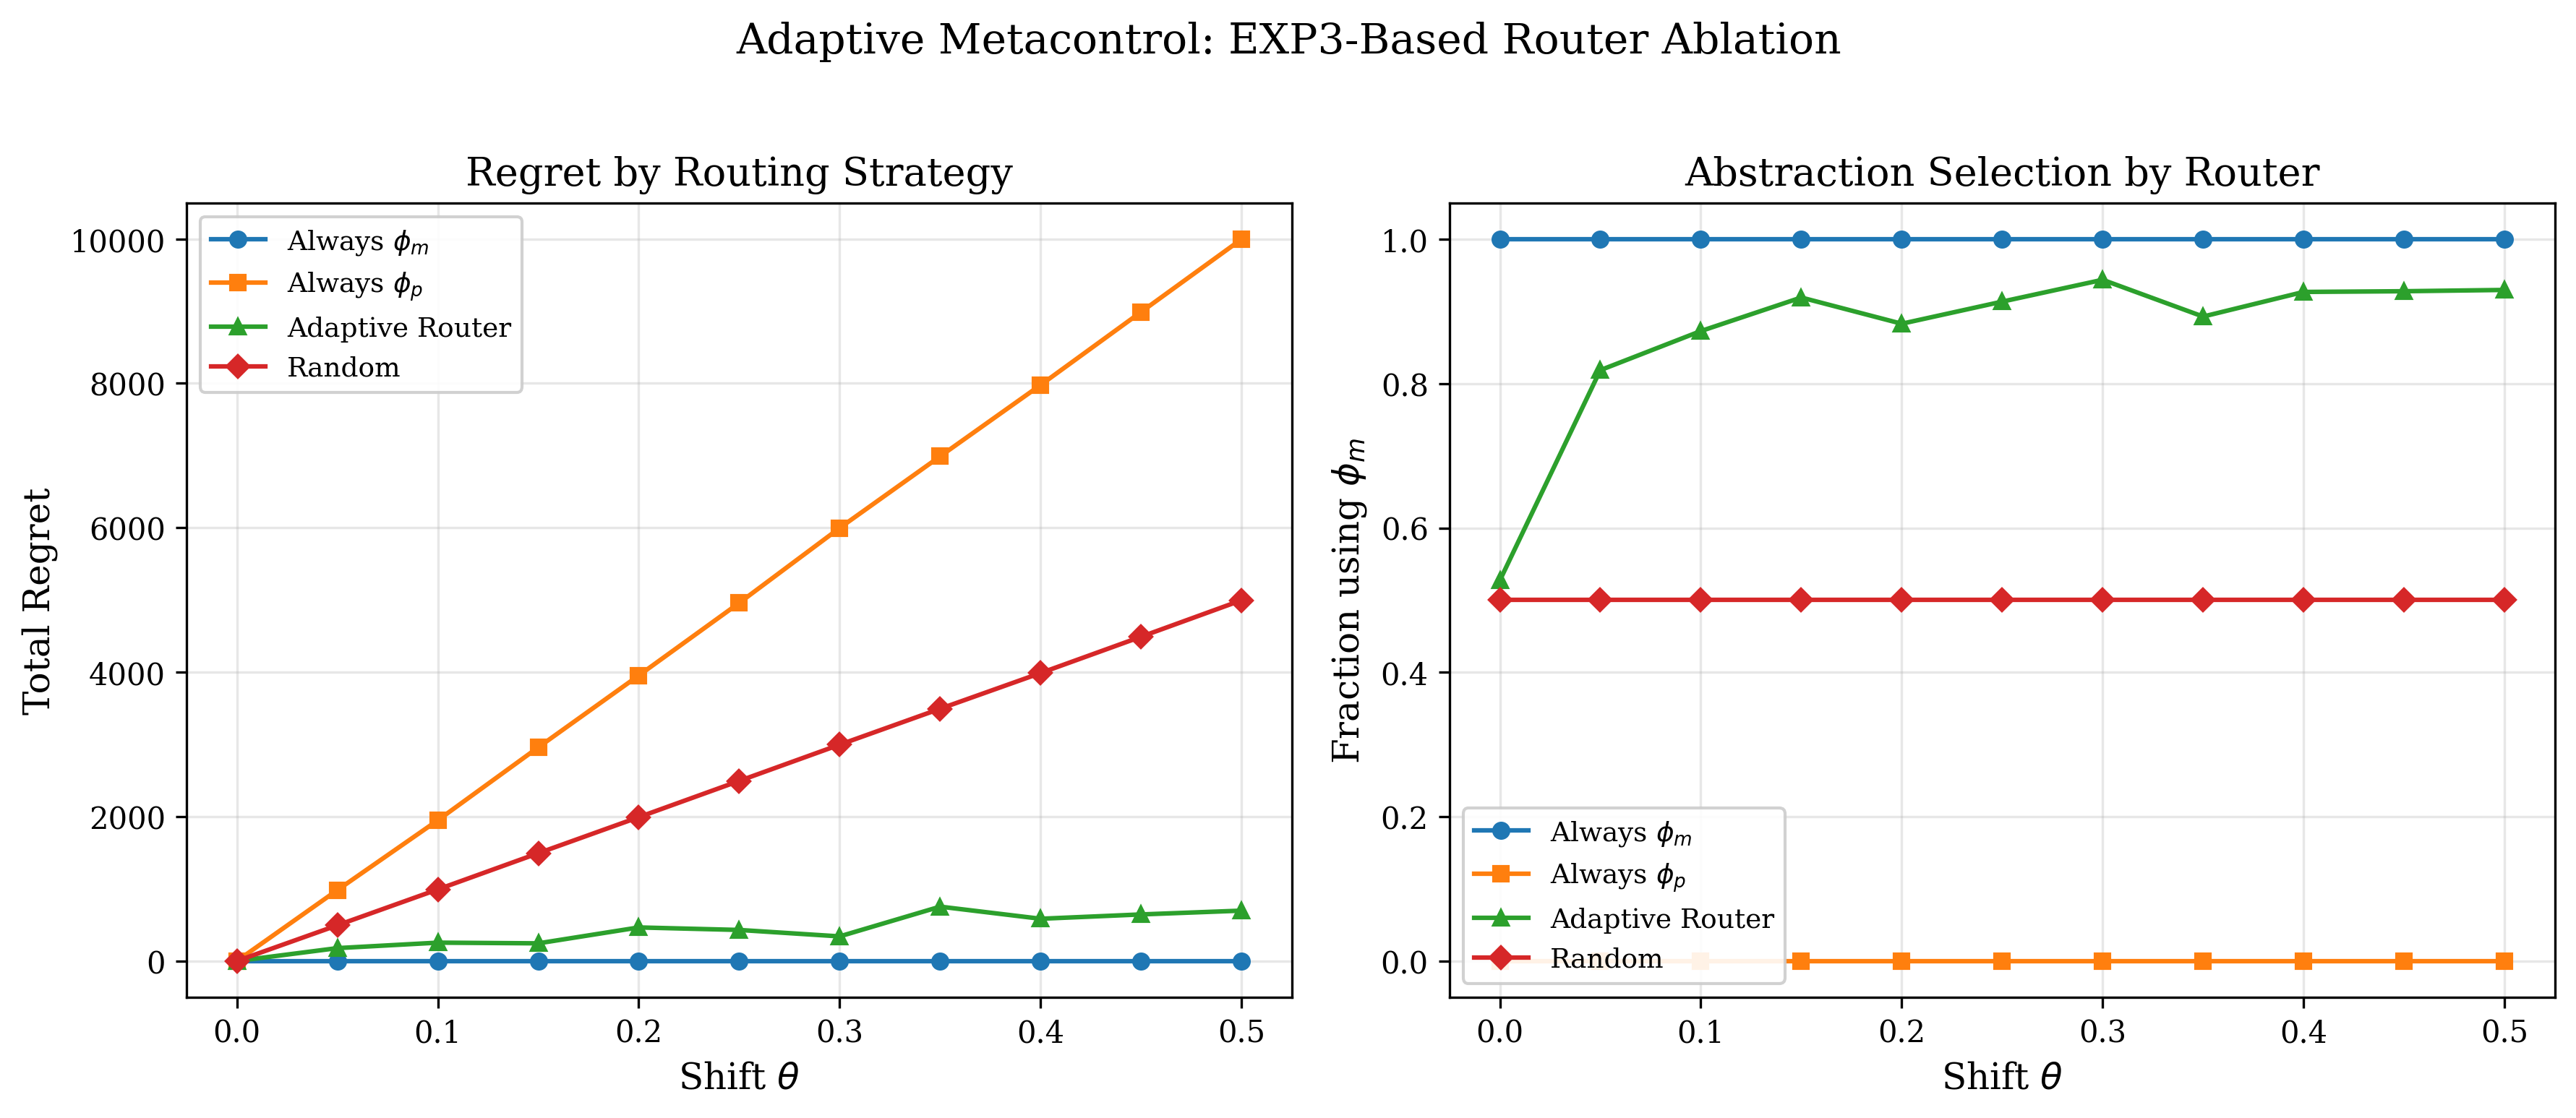
\includegraphics[width=\textwidth]{fig7_router_ablation.png}
    \caption{Router ablation. Left: total regret by strategy. Right: fraction of steps using $\phim$. The adaptive router learns to select $\phim$ as shift increases.}
    \label{fig:router}
\end{figure}

% ==================================================================
% 7. DISCUSSION
% ==================================================================
\section{Discussion}
\label{sec:discussion}

\paragraph{Why learned representations fail.} The core issue is that predictive sufficiency at source does \emph{not} imply mechanism invariance. All six GPU baselines optimize for source-distribution objectives (bisimulation distance, reconstruction, next-latent prediction). Since $S_1$ and $S_2$ carry identical information at source, these objectives cannot distinguish causal from effectual variables. The learned representations inevitably absorb both, and the effectual components degrade under shift.

\paragraph{The Qwen3 phenomenon.} Qwen3-235B's blackbox behavior is particularly striking: it achieves 100\% $S_2$-match at $\theta = 0.5$, meaning it has learned a \emph{pure} $\phip$ strategy from its pretraining. When told ``two binary values,'' Qwen3 consistently selects the second value---a pattern likely absorbed from training data where the second listed value is often the ``answer.'' This provides a concrete example of how pretraining biases can manifest as predictive (rather than causal) reasoning strategies.

\paragraph{Implications for AGI.} The separation theorem reveals a fundamental tension in transfer-robust intelligence: observational data alone cannot distinguish causal from correlational features. This has direct implications for systems aspiring to general intelligence:
\begin{itemize}
    \item \textbf{Architecture}: Learned world models (regardless of whether they use reconstruction, JEPA, or bisimulation objectives) converge to predictive representations. Achieving mechanism invariance may require explicit causal structure discovery or privileged knowledge.
    \item \textbf{Metacognition}: The success of the adaptive router suggests that a form of metacognitive monitoring---detecting when learned abstractions fail and switching to alternatives---may be a practical path toward robust transfer.
    \item \textbf{Knowledge representation}: The LLM results show that explicit causal descriptions (``$S_1$ causes $S_2$'') are sufficient for perfect transfer. This underscores the value of symbolic causal knowledge alongside statistical learning.
\end{itemize}

\paragraph{Limitations.} Our environments are deliberately minimal: binary state spaces, i.i.d.\ dynamics, and 2-component causal structures. This is by design---the separation theorem is a \emph{lower bound} argument showing that the problem exists even in the simplest possible setting. Scaling to high-dimensional, temporally correlated environments is an important direction for future work. Additionally, the LLM experiments evaluate single-step decisions rather than sequential planning, and the GPU baselines use simplified implementations rather than full-scale architectures.

% ==================================================================
% 8. CONCLUSION
% ==================================================================
\section{Conclusion}
\label{sec:conclusion}

We have established a separation theorem demonstrating that two observationally equivalent abstractions can have a $\Theta(\theta \cdot T)$ regret gap under graph-preserving shift, formalized the counterfactual cost of mechanism invariance, and validated the separation across 15 baselines from three distinct paradigms. The results reveal that standard representation-learning objectives are insufficient for transfer robustness, that LLMs with causal knowledge can achieve mechanism-invariant behavior, and that adaptive metacontrol offers a practical bridge.

\paragraph{Future work.} Key directions include: (1) extending the CausalShift benchmark to continuous, high-dimensional state spaces; (2) developing representation-learning objectives that provably achieve mechanism invariance; (3) scaling the adaptive router to larger abstraction families; and (4) investigating whether LLMs can discover causal structure from interaction data (rather than from privileged descriptions).

% ==================================================================
% REFERENCES
% ==================================================================
\begin{thebibliography}{99}

\bibitem{abel2018state}
Abel, D., Hershkowitz, D.E., Littman, M.L.:
Near optimal behavior via approximate state abstraction.
In: International Conference on Machine Learning, pp.~2915--2923. PMLR (2018)

\bibitem{arjovsky2019invariant}
Arjovsky, M., Bottou, L., Gulchanani, I., Lopez-Paz, D.:
Invariant risk minimization.
arXiv preprint arXiv:1907.02893 (2019)

\bibitem{auer2002nonstochastic}
Auer, P., Cesa-Bianchi, N., Freund, Y., Schapire, R.E.:
The nonstochastic multiarmed bandit problem.
SIAM Journal on Computing \textbf{32}(1), 48--77 (2002)

\bibitem{ferns2004metrics}
Ferns, N., Panangaden, P., Precup, D.:
Metrics for finite Markov decision processes.
In: Proceedings of the 20th Conference on Uncertainty in Artificial Intelligence, pp.~162--169 (2004)

\bibitem{hafner2023mastering}
Hafner, D., Pasukonis, J., Ba, J., Lillicrap, T.:
Mastering diverse domains through world models.
arXiv preprint arXiv:2301.04104 (2023)

\bibitem{huang2022language}
Huang, W., Abbeel, P., Pathak, D., Mordatch, I.:
Language models as zero-shot planners: Extracting actionable knowledge for embodied agents.
In: International Conference on Machine Learning, pp.~9118--9147. PMLR (2022)

\bibitem{li2006towards}
Li, L., Walsh, T.J., Littman, M.L.:
Towards a unified theory of state abstraction for MDPs.
In: International Symposium on Artificial Intelligence and Mathematics (2006)

\bibitem{peters2016causal}
Peters, J., B{\"u}hlmann, P., Meinshausen, N.:
Causal inference by using invariant prediction: Identification and confidence intervals.
Journal of the Royal Statistical Society: Series B \textbf{78}(5), 947--1012 (2016)

\bibitem{scholkopf2021toward}
Sch{\"o}lkopf, B., Locatello, F., Bauer, S., Ke, N.R., Kalchbrenner, N., Goyal, A., Bengio, Y.:
Toward causal representation learning.
Proceedings of the IEEE \textbf{109}(5), 612--634 (2021)

\bibitem{valmeekam2023planning}
Valmeekam, K., Marquez, M., Sreedharan, S., Kambhampati, S.:
On the planning abilities of large language models.
In: Advances in Neural Information Processing Systems, vol.~36 (2023)

\bibitem{wang2024building}
Wang, Z., Xiao, C., Xu, Z., Zhu, Y.:
Building minimal and reusable causal state abstractions for reinforcement learning.
arXiv preprint arXiv:2401.12497 (2024)

\bibitem{zenke2026reconstruction}
Zenke Lab.:
Reconstruction-free world models match DreamerV3 performance.
arXiv preprint arXiv:2603.07083 (2026)

\bibitem{zhang2021learning}
Zhang, A., McAllister, R., Calandra, R., Gal, Y., Levine, S.:
Learning invariant representations for reinforcement learning without reconstruction.
In: International Conference on Learning Representations (2021)

\end{thebibliography}

\end{document}
